% Settings for the default beamer theme
\documentclass[english, aspectratio=169]{beamer}
\usepackage[T1]{fontenc}
\usepackage[utf8]{inputenc}
\usepackage{adjustbox}
\usepackage{tabularx}
\usepackage{listings}
\usepackage{graphicx}
\usepackage{array}
\usepackage{babel}
\usepackage[ruled,vlined]{algorithm2e}
\usepackage{blkarray}
\SetAlgorithmName{Algoritmus}{algoritmus}{List of Algorithms}
\setcounter{secnumdepth}{3}
\setcounter{tocdepth}{3}


\makeatletter

\newcommand\makebeamertitle{\frame{\maketitle}}

% (ERT) argument for the TOC
\AtBeginDocument{%
  \let\origtableofcontents=\tableofcontents
  \def\tableofcontents{\@ifnextchar[{\origtableofcontents}{\gobbletableofcontents}}
  \def\gobbletableofcontents#1{\origtableofcontents}
}

% Theme settings
\usetheme{Frankfurt}
\usecolortheme{default}
\usefonttheme[onlymath]{serif}

% Template settings
\setbeamertemplate{navigation symbols}{}
\setbeamertemplate{blocks}[rounded][shadow=false]
\setbeamertemplate{title page}[default][colsep=-4bp, rounded=true, shadow=false]
\makeatother

% Custom color definitions
\definecolor{lightgrey}{gray}{0.95}
\definecolor{DarkerGreen}{RGB}{0,85,0} % Adjust the RGB values as needed

% Use the newly defined color in Beamer theme elements
\setbeamercolor{structure}{fg=DarkerGreen} % Changes basic structural elements to Darker Green
\setbeamercolor{title in head/foot}{bg=DarkerGreen} % Changes the title in header/footer to Darker Green

% Definitions for program code sections
\lstset{
	language=bash,
	basicstyle=\ttfamily\footnotesize, % Monospace font
	backgroundcolor=\color{lightgrey}, % Background color
	frame=single, % Frame around the code
	keywordstyle=\color{black}, % Keywords color
	commentstyle=\color{black}, % Comments color
	stringstyle=\color{red}, % Strings color
	showstringspaces=false, % Do not show spaces in strings
	breaklines=true, % Automatically break long lines
}

\lstset{
	language=python,
	basicstyle=\ttfamily\scriptsize, % Basic font style
	keywordstyle=\bfseries\color{blue}, % Keywords in bold and blue
	stringstyle=\color{red}, % Strings in red
	commentstyle=\color{green!50!black}, % Comments in green
	showstringspaces=false, % Do not show spaces in strings
	numbers=left, % Line numbers on the left
	numberstyle=\tiny\color{gray}, % Line number style
	stepnumber=1, % Line number step
	numbersep=5pt, % Distance of line numbers from code
	frame=single, % Frame around the code
	rulecolor=\color{black}, % Frame color
	tabsize=2, % Tab size
	breaklines=true, % Automatic line breaking
	breakatwhitespace=false, % Break lines at whitespace
	captionpos=b, % Caption position
	escapeinside={\%*}{*)}, % Escape to LaTeX
	morekeywords={self}, % Additional keywords
	literate={á}{{\'a}}1
	{é}{{\'e}}1
	{í}{{\'i}}1
	{ó}{{\'o}}1
	{ú}{{\'u}}1
	{ő}{{\H{o}}}1
	{ű}{{\H{u}}}1
	{Á}{{\'A}}1
	{É}{{\'E}}1
	{Í}{{\'I}}1	
	{Ó}{{\'O}}1	
	{Ú}{{\'U}}1
	{Ő}{{\H{O}}}1
	{Ű}{{\H{U}}}1
	{Ö}{{\"O}}1
	{Ü}{{\"U}}1
	{ö}{{\"o}}1
	{ü}{{\"u}}1
}


\begin{document}

% Title page
\section{Bevezetés}
\title[]{Adatbányászat a Gyakorlatban}
\subtitle{5. Gyakorlat: Gyakorisági adatok kezelése}
\author[Kuknyó Dániel]{Kuknyó Dániel\\Budapesti Gazdasági Egyetem}
\date{2024/25\\1.félév}
\makebeamertitle

% Table of contents slide
\begin{frame}
\tableofcontents{}
\end{frame}

% Table of contents of the current section
\begin{frame}
\tableofcontents[currentsection]
\end{frame}

\begin{frame}[fragile]{Hisztogramok létrehozása}
	\begin{columns}
		\begin{column}{.5\textwidth}
			\begin{block}{Hisztogram}
				A hisztogram egy statisztikai grafikon, amely az adatok eloszlását mutatja be. Oszlopdiagram formájában ábrázolja, hogy az adatok milyen gyakorisággal fordulnak elő különböző intervallumokban.
			\end{block}
			\medskip
			Hisztogram létrehozása plotly segítségével:
			\begin{lstlisting}[language=python]
px.histogram(data_frame=df, x=gini)
			\end{lstlisting}
		\end{column}
		\begin{column}{.5\textwidth}
			\begin{center}
				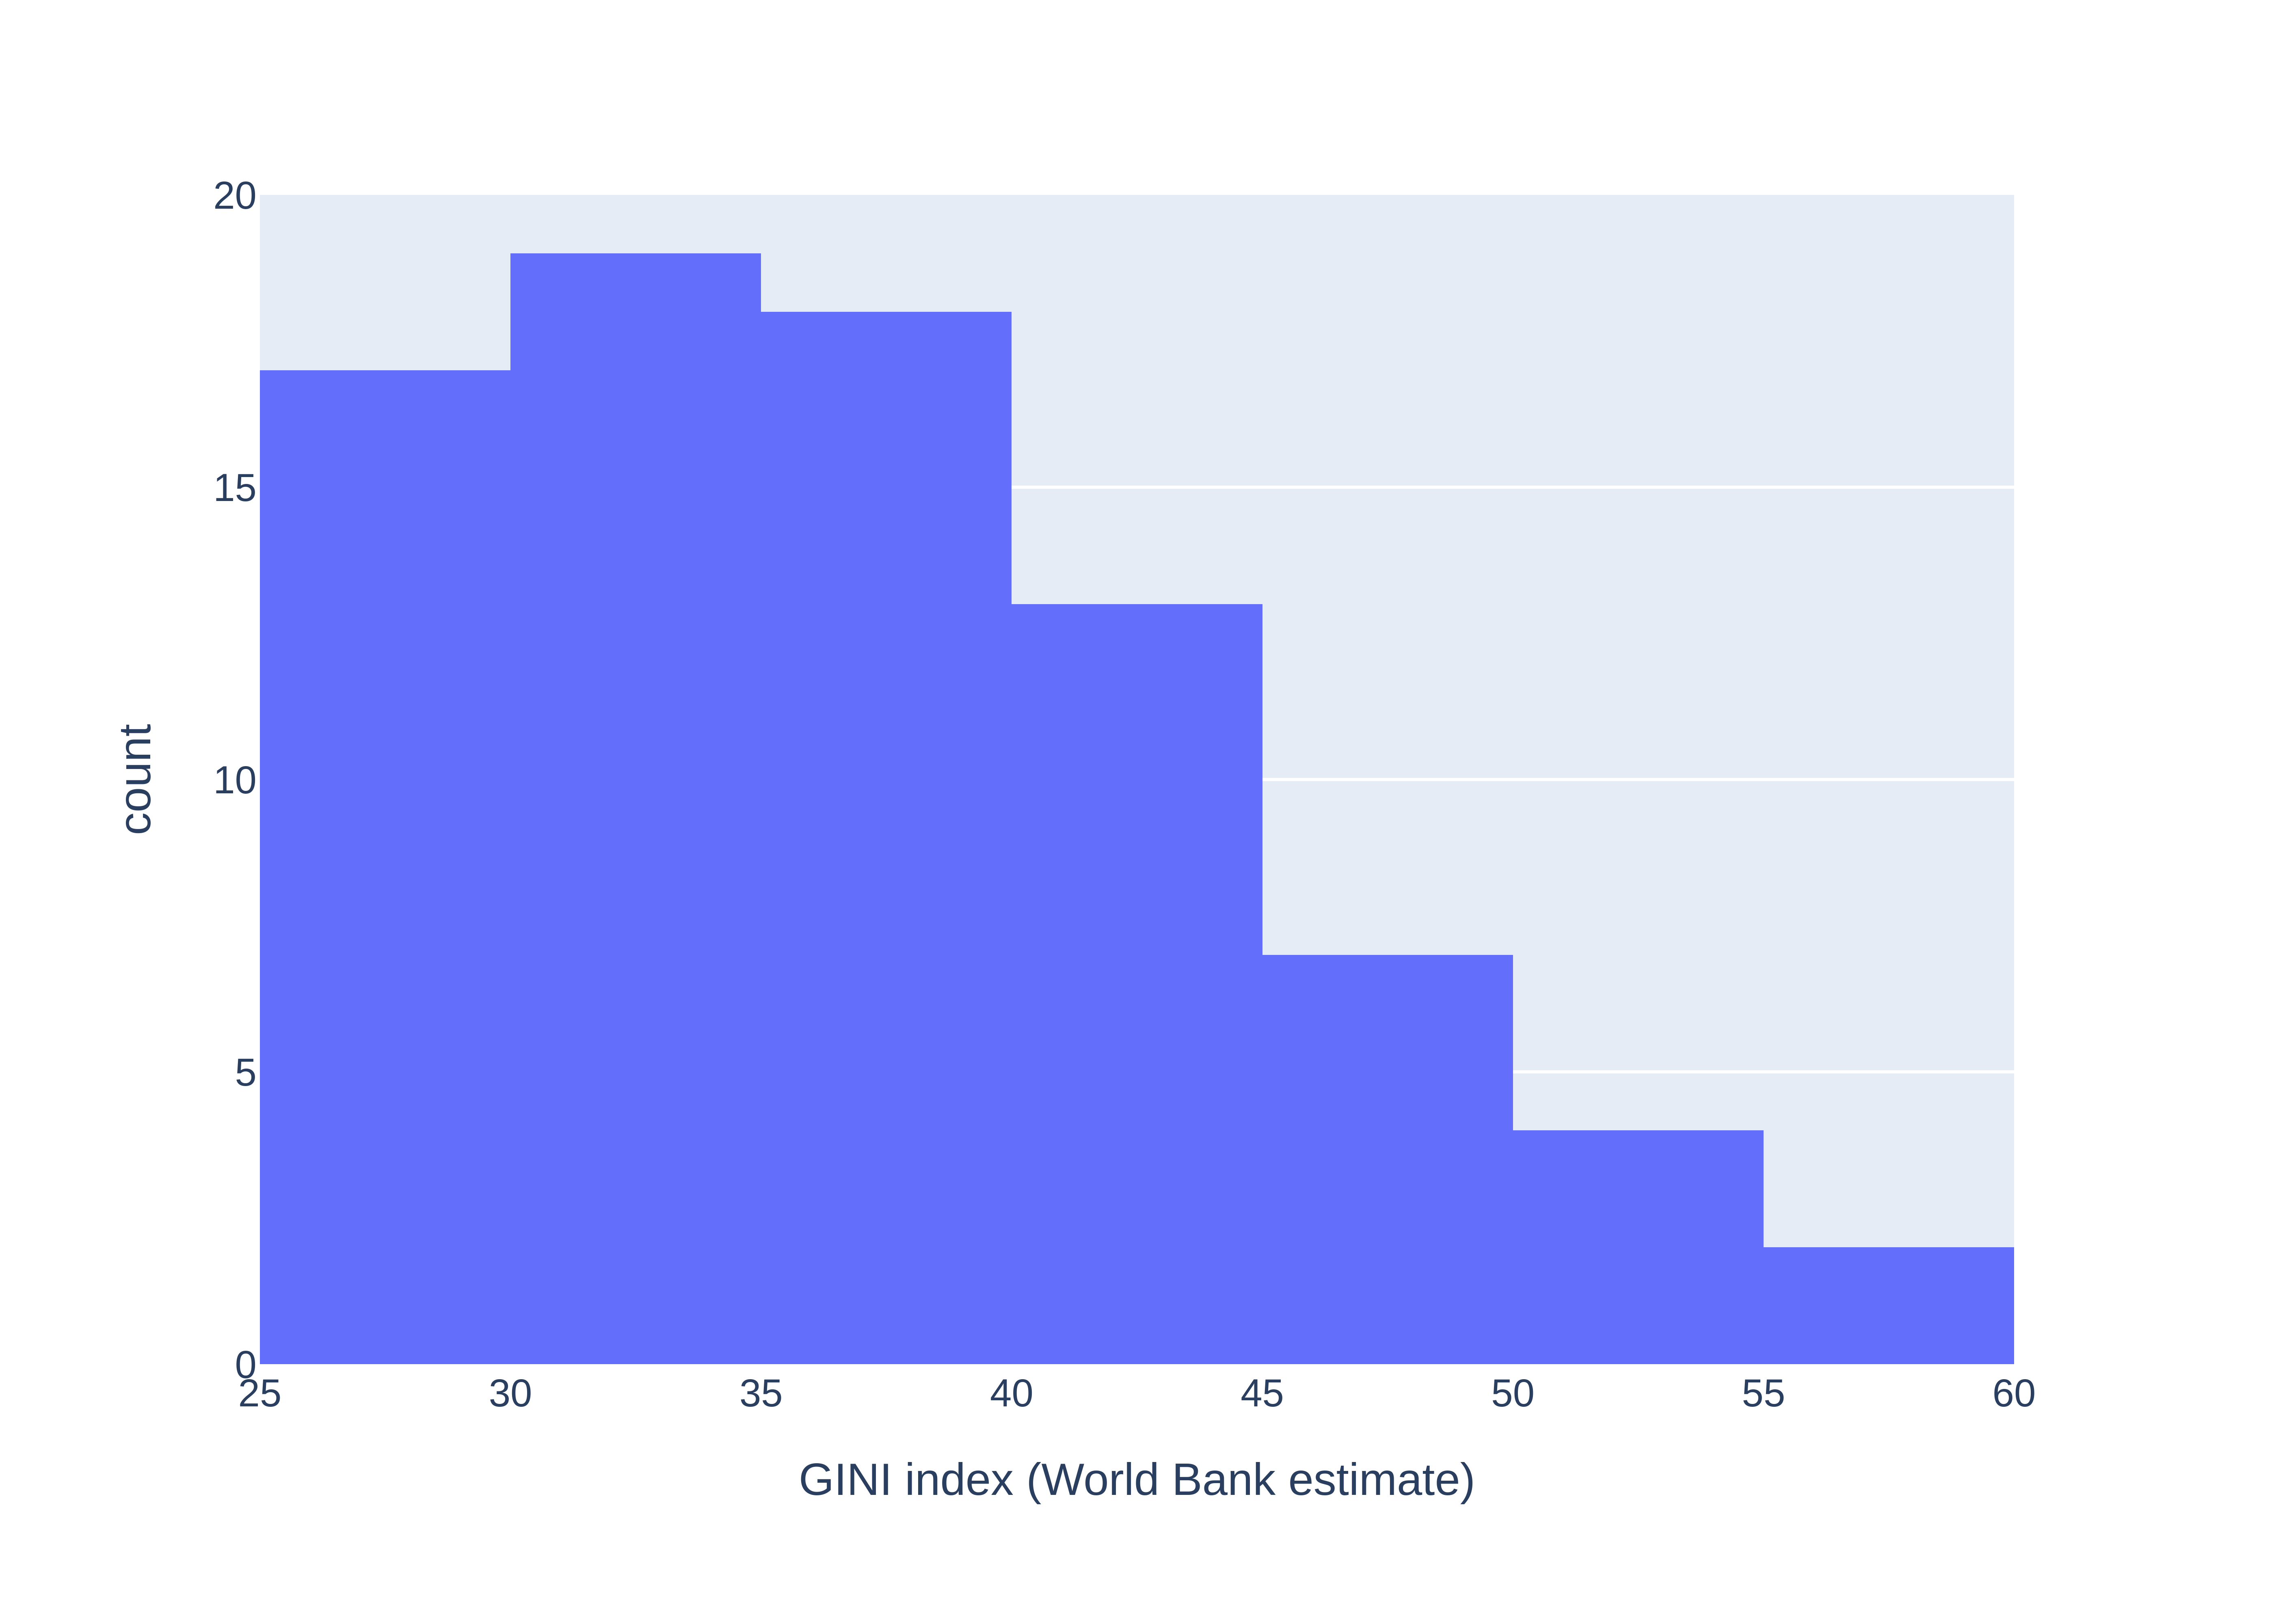
\includegraphics[width=7cm, height=7cm, keepaspectratio]{images/freq_1.png}
			\end{center}
		\end{column}
	\end{columns}
\end{frame}

\begin{frame}[fragile]{Hisztogramok felbontása}
	\begin{columns}
		\begin{column}{.5\textwidth}
			\begin{block}{Osztályköz}
				Az osztályközök határozzák meg, hogy az adatok milyen tartományokba kerülnek, és ezek az intervallumok határozzák meg a hisztogram oszlopainak szélességét.
			\end{block}
			\medskip
			Az osztályközök száma az \texttt{nbins} paraméter segítségével állítható. 
			\begin{lstlisting}[language=python]
for n in [2, 45, 500]:
	px.histogram(data_frame=df, x=gini, nbins=n)
			\end{lstlisting}
		\end{column}
		\begin{column}{.5\textwidth}
			\begin{center}
				\includegraphics<1>[width=7cm, height=7cm, keepaspectratio]{images/freq_2.png}
				\includegraphics<2>[width=7cm, height=7cm, keepaspectratio]{images/freq_3.png}
				\includegraphics<3>[width=7cm, height=7cm, keepaspectratio]{images/freq_4.png}
			\end{center}
		\end{column}
	\end{columns}
\end{frame}

\begin{frame}[fragile]{Hisztogram hasítása színekkel}
	\begin{columns}
		\begin{column}{.5\textwidth}
			Plotly express diagramokat lehetséges változón belüli csoportonként meghasítani. Ennek eléréséhez a \texttt{color} paramétert kell a megfelelő változóra állítani.\par\medskip
			\begin{lstlisting}[language=python]
px.histogram(data_frame=df, x=gini, color='Income Group', color_discrete_sequence=px.colors.qualitative.Set1)
			\end{lstlisting}
		\end{column}
		\begin{column}{.5\textwidth}
			\begin{center}
				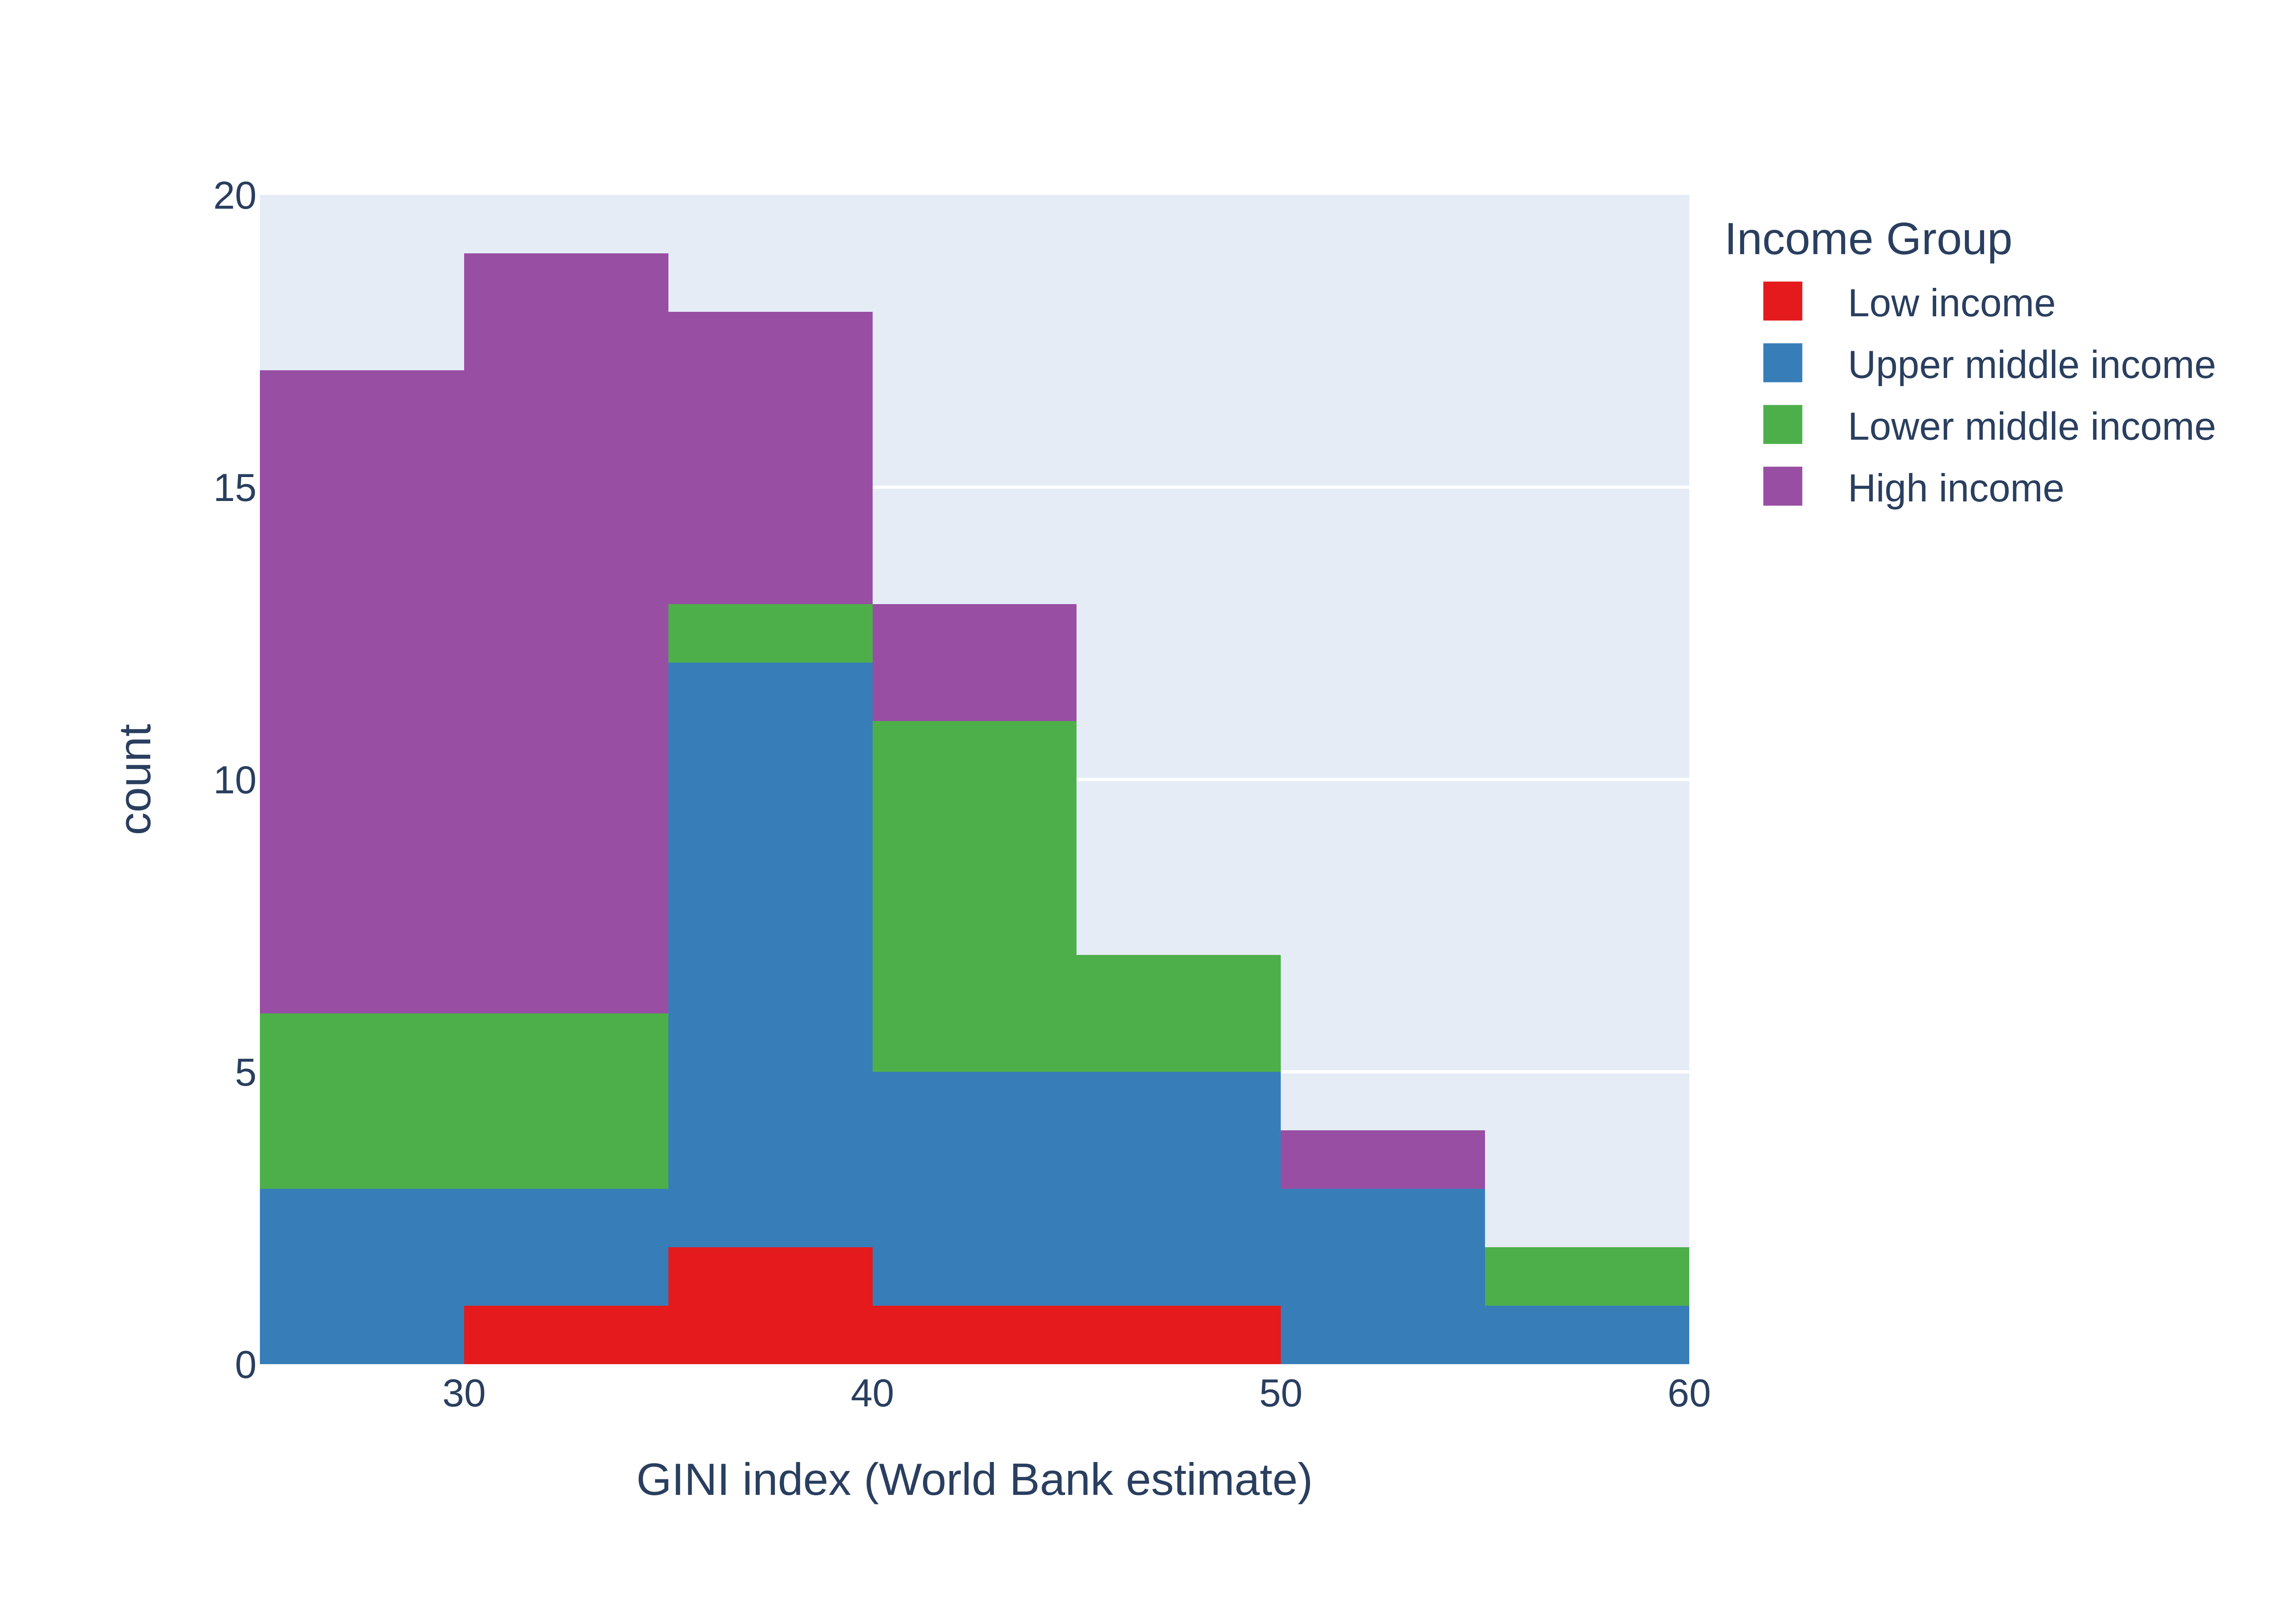
\includegraphics[width=7cm, height=7cm, keepaspectratio]{images/freq_5.png}
			\end{center}
		\end{column}
	\end{columns}
\end{frame}

\begin{frame}[fragile]{Csoportosított hisztogramok}
	\begin{columns}
		\begin{column}{.5\textwidth}
			Vannak olyan esetek, amikor egy változónak több csoportját egymás mellett szükséges megmutatni. Ekkor a hisztogramokat lehetséges csoportosítani adott értékek szerint, a \texttt{color} és a \texttt{barmode='group'} paraméterek állításával.\par\medskip
			\begin{lstlisting}[language=python]
px.histogram(df, x=gini, color='year', barmode='group')
			\end{lstlisting}
		\end{column}
		\begin{column}{.5\textwidth}
			\begin{center}
				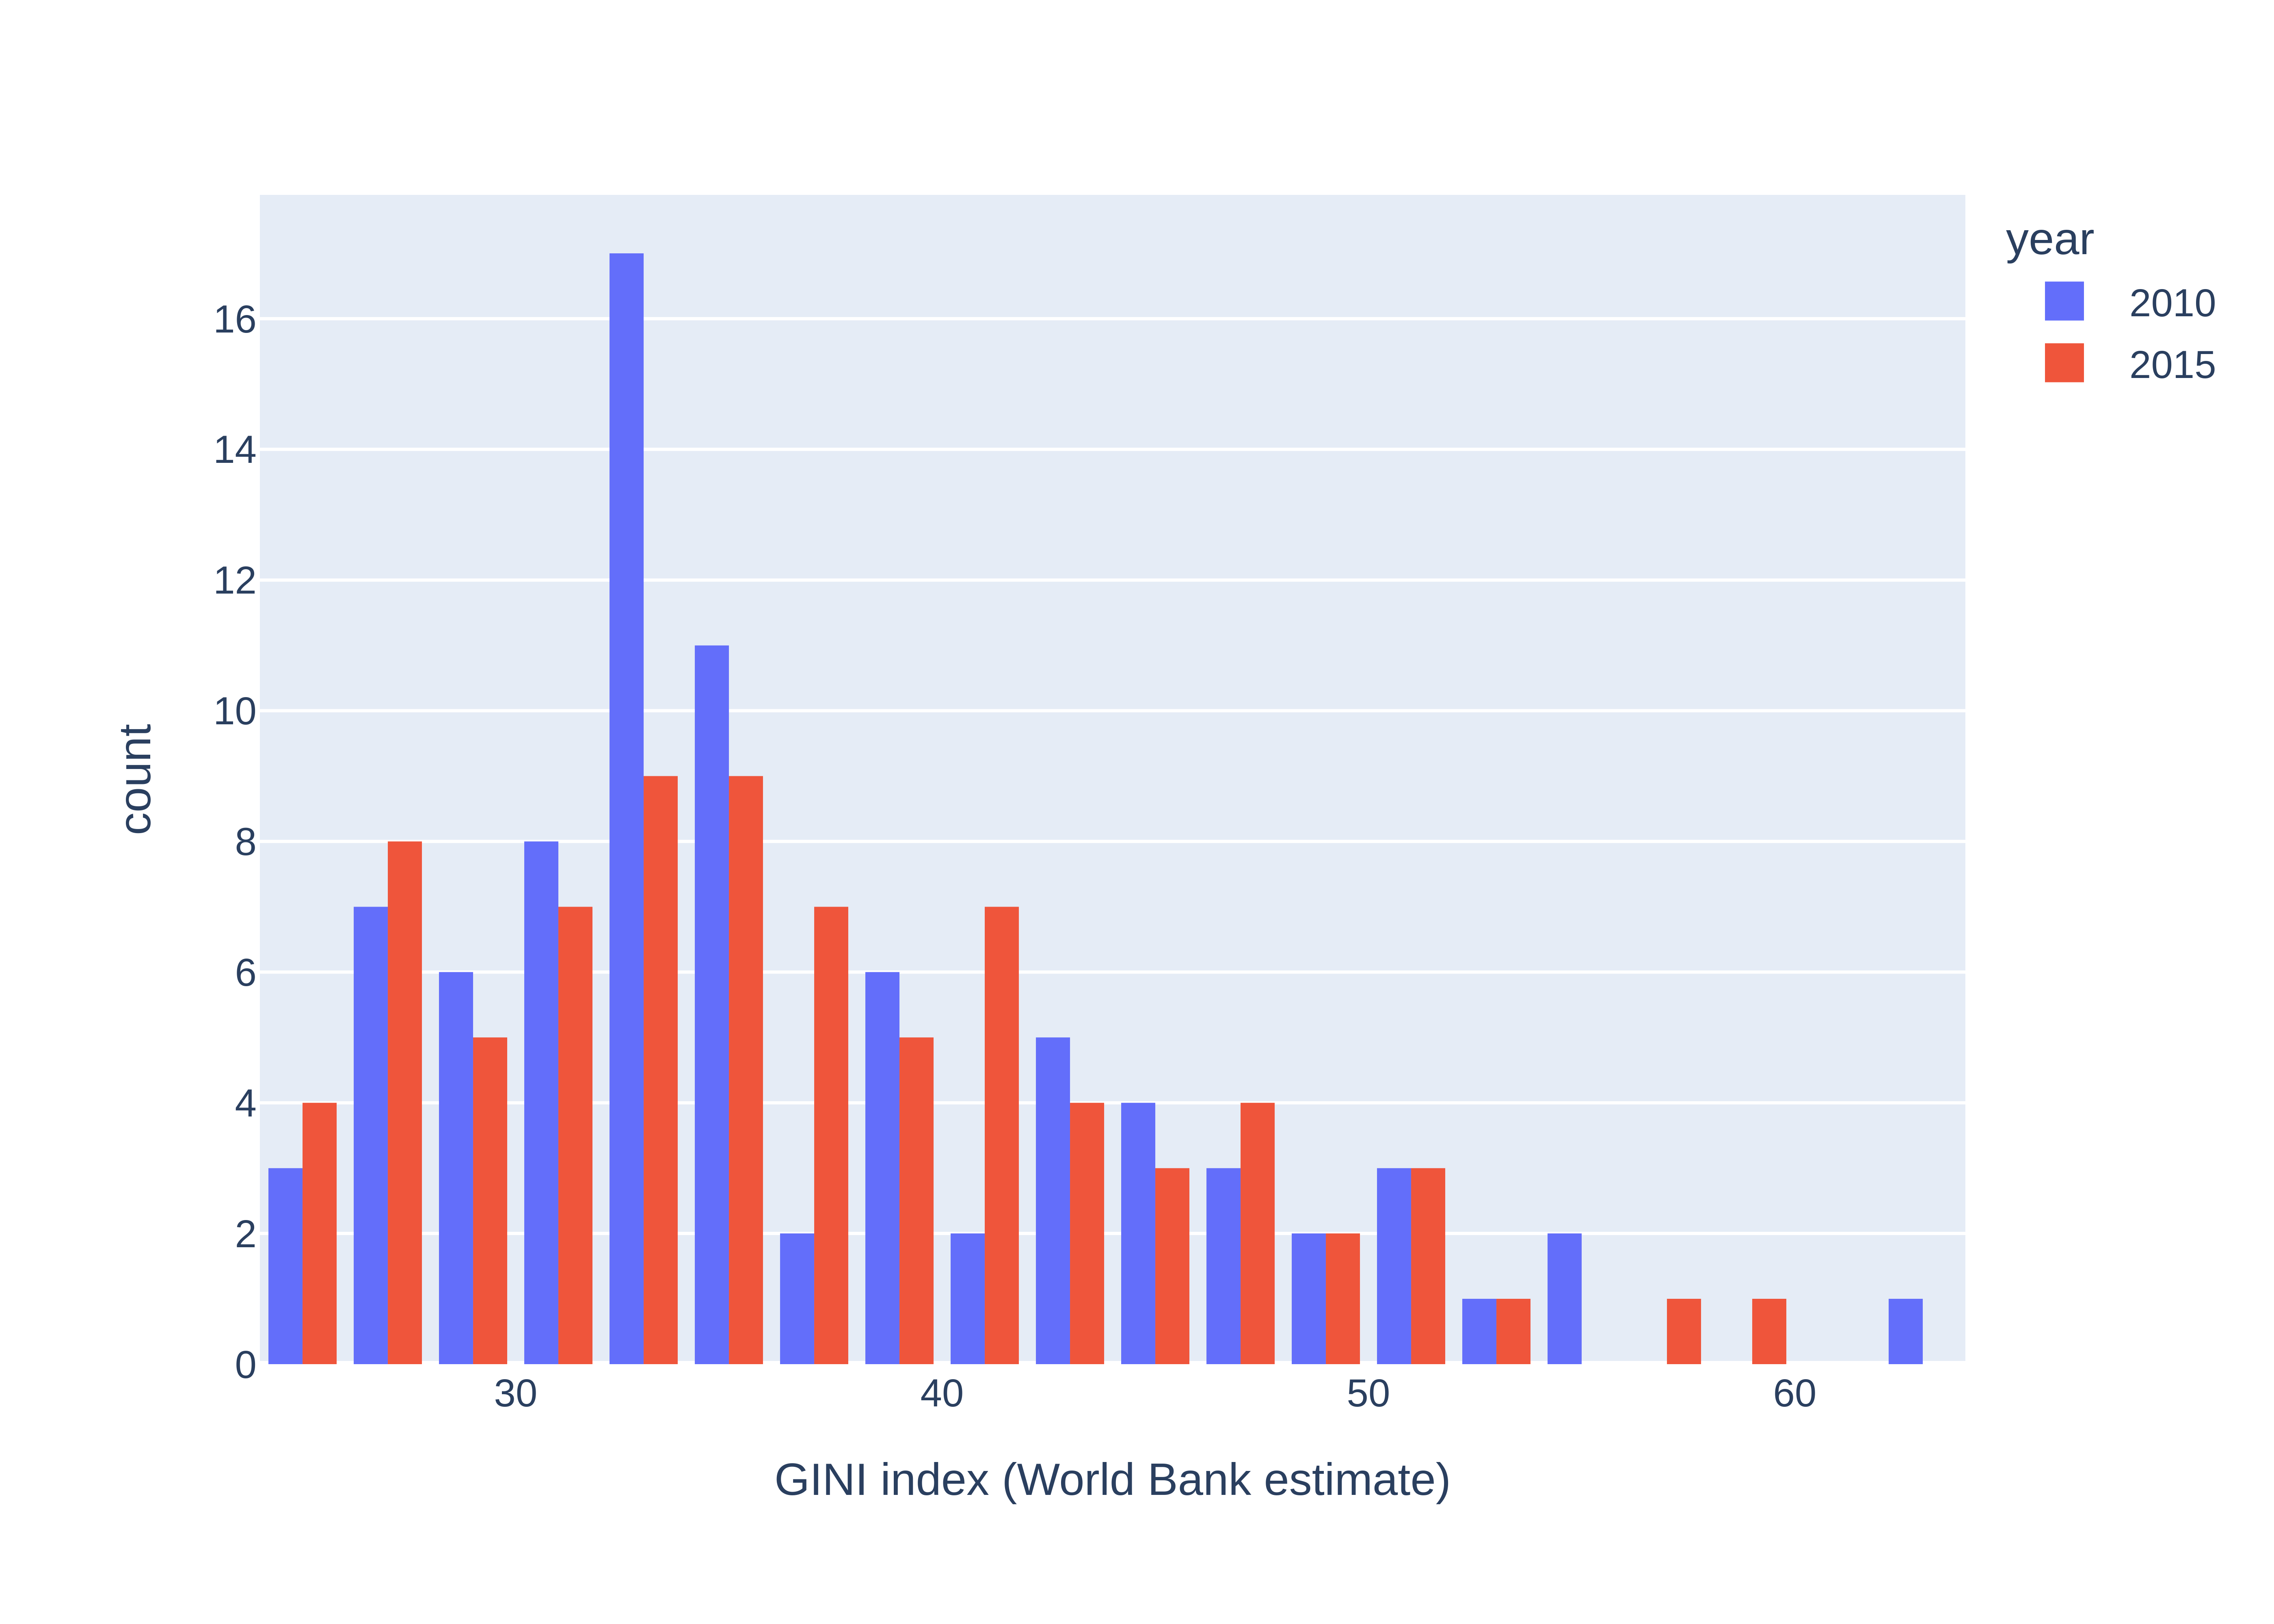
\includegraphics[width=7cm, height=7cm, keepaspectratio]{images/freq_6.png}
			\end{center}
		\end{column}
	\end{columns}
\end{frame}

\begin{frame}[fragile]{Hasított hisztogramok}
	\begin{columns}
		\begin{column}{.5\textwidth}
			A diagramok hasítása adott változó értékei szerint lehetséges úgy is, hogy minden, a változóhoz tartozó értékre szűrt adathalmaz egy külön diagramon jelenik meg, a \texttt{facet\_col} paraméter állításával.\par\medskip
			\begin{lstlisting}[language=python]
px.histogram(df, x=gini, color='year', facet_col='year')
			\end{lstlisting}
		\end{column}
		\begin{column}{.5\textwidth}
			\begin{center}
				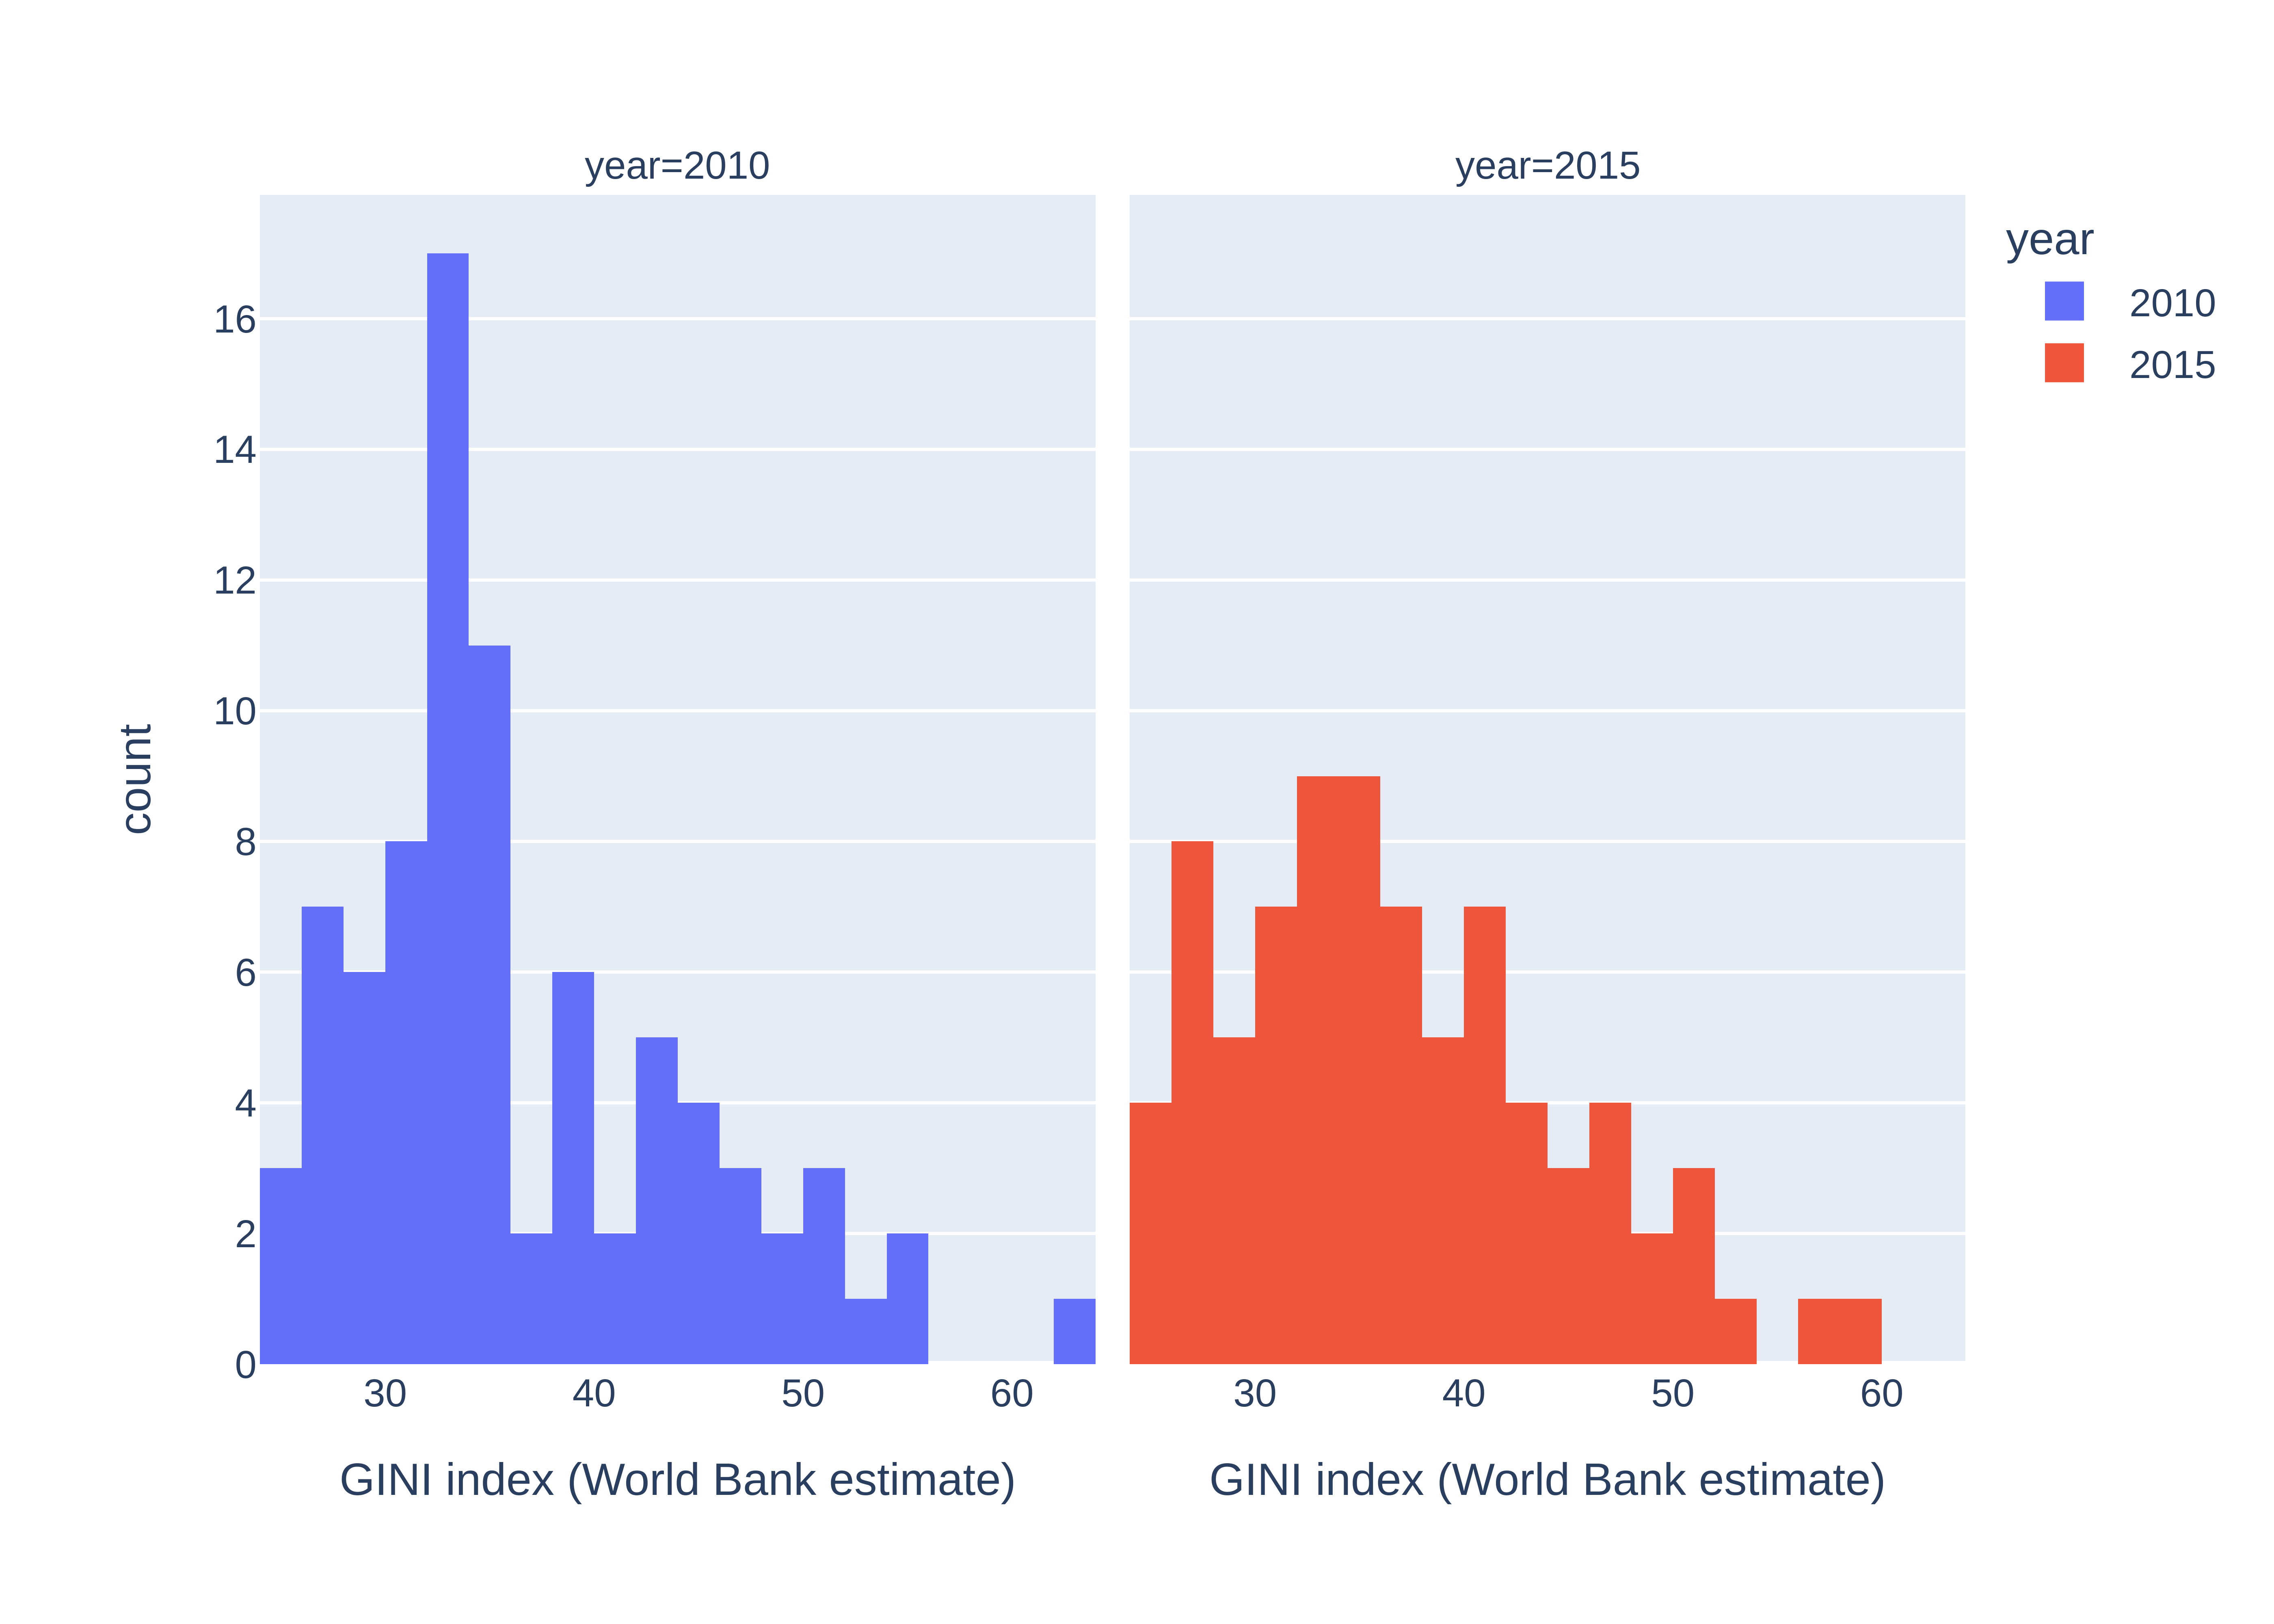
\includegraphics[width=7cm, height=7cm, keepaspectratio]{images/freq_7.png}
			\end{center}
		\end{column}
	\end{columns}
\end{frame}

\begin{frame}[fragile]{Hisztogramok normalizálása}
	\begin{columns}
		\begin{column}{.5\textwidth}
			\begin{block}{Normalizált hisztogram}
				Olyan grafikon, ahol az egyes oszlopok az adott intervallumba eső adatok gyakoriságát jelzi olyan módon, hogy az oszlopok összege 1 legyen. 
			\end{block}
			\begin{lstlisting}[language=python]
fig = px.histogram(df, x=gini, color='year', facet_col='year')
fig.layout.yaxis.ticksuffix = '%'
fig.layout.yaxis.title = 'Százalékos gyakoriság'
fig.show()
			\end{lstlisting}
		\end{column}
		\begin{column}{.5\textwidth}
			\begin{center}
				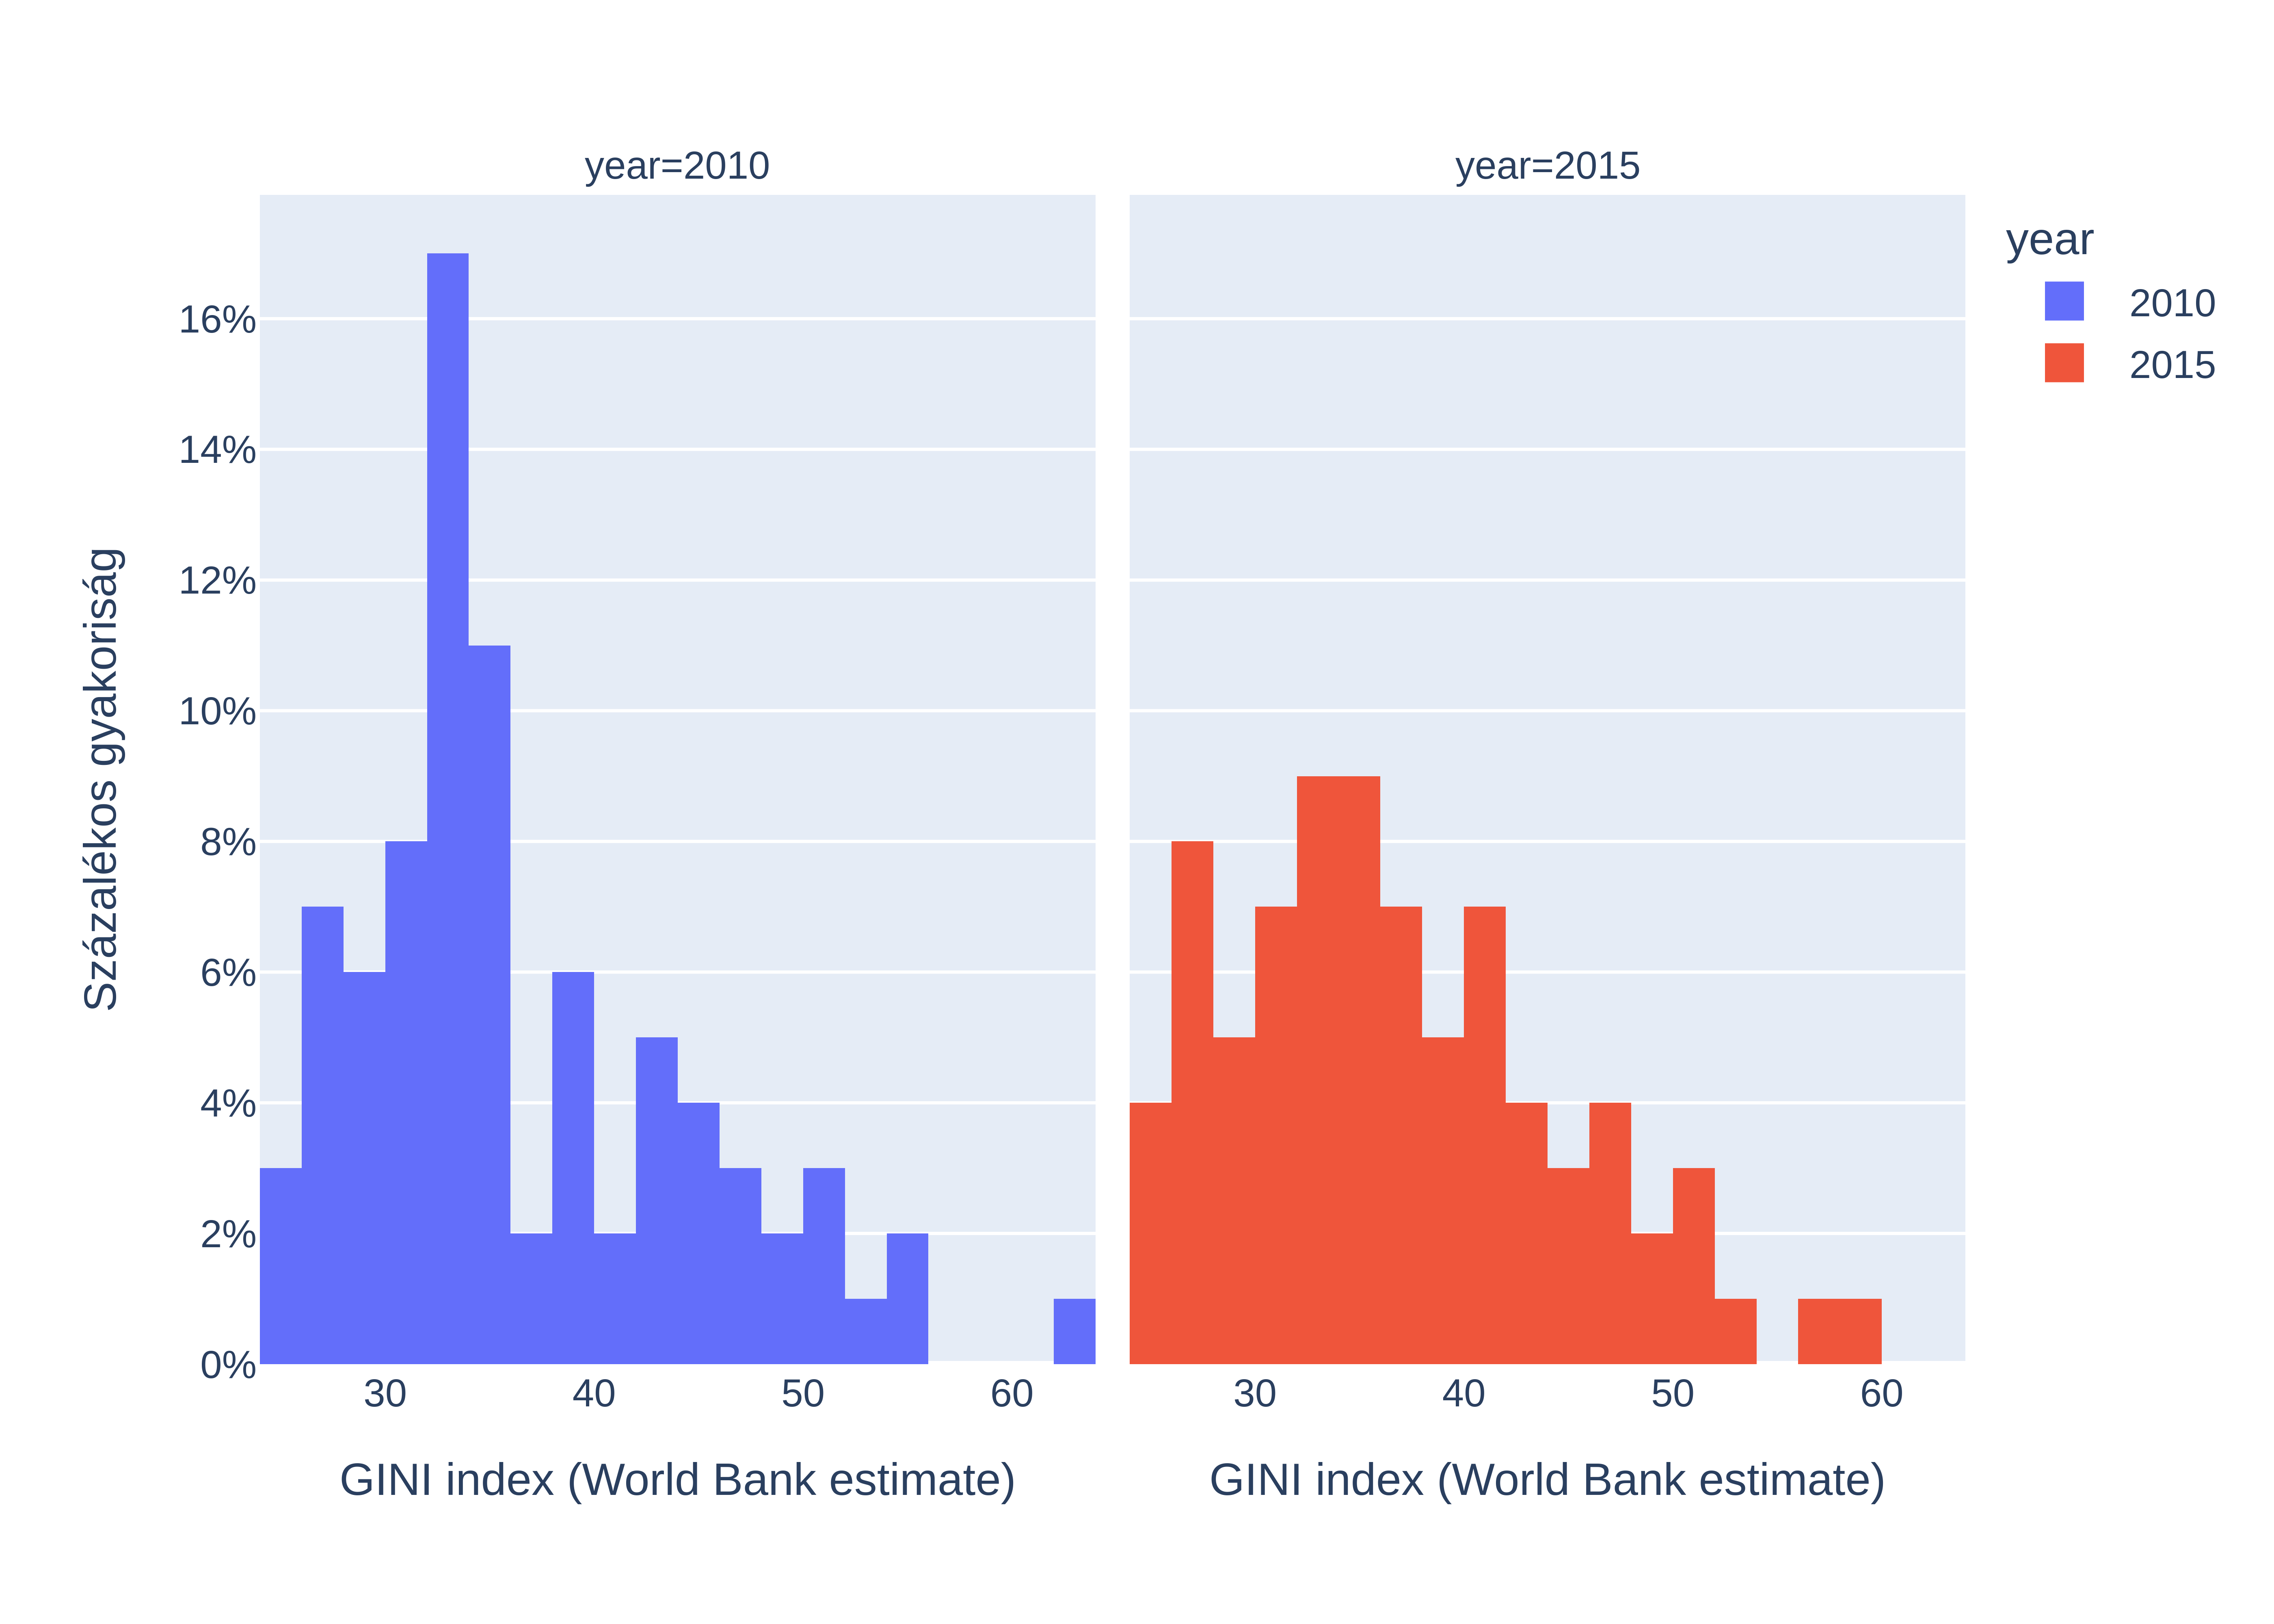
\includegraphics[width=7cm, height=7cm, keepaspectratio]{images/freq_8.png}
			\end{center}
		\end{column}
	\end{columns}
\end{frame}

\begin{frame}{Alkalmazás interaktív hisztogramokkal (\texttt{freq\_app\_v1.py})}
	\begin{columns}
		\begin{column}{.5\textwidth}
			A callback függvények a felhasználói interakciók alapján frissítik a grafikonokat. A \texttt{display\_histogram} függvény három bemeneti elemet figyel \texttt{(years, indicator, bins)}, és ezek alapján frissíti a hisztogram ábrát.\par\medskip
			Ha nincs kiválasztott év vagy indikátor, a függvény nem frissíti az ábrát (\texttt{PreventUpdate}). Az adatok szűrése után a Plotly Express segítségével készül el a hisztogram.
		\end{column}
		\begin{column}{.5\textwidth}
			\begin{center}
				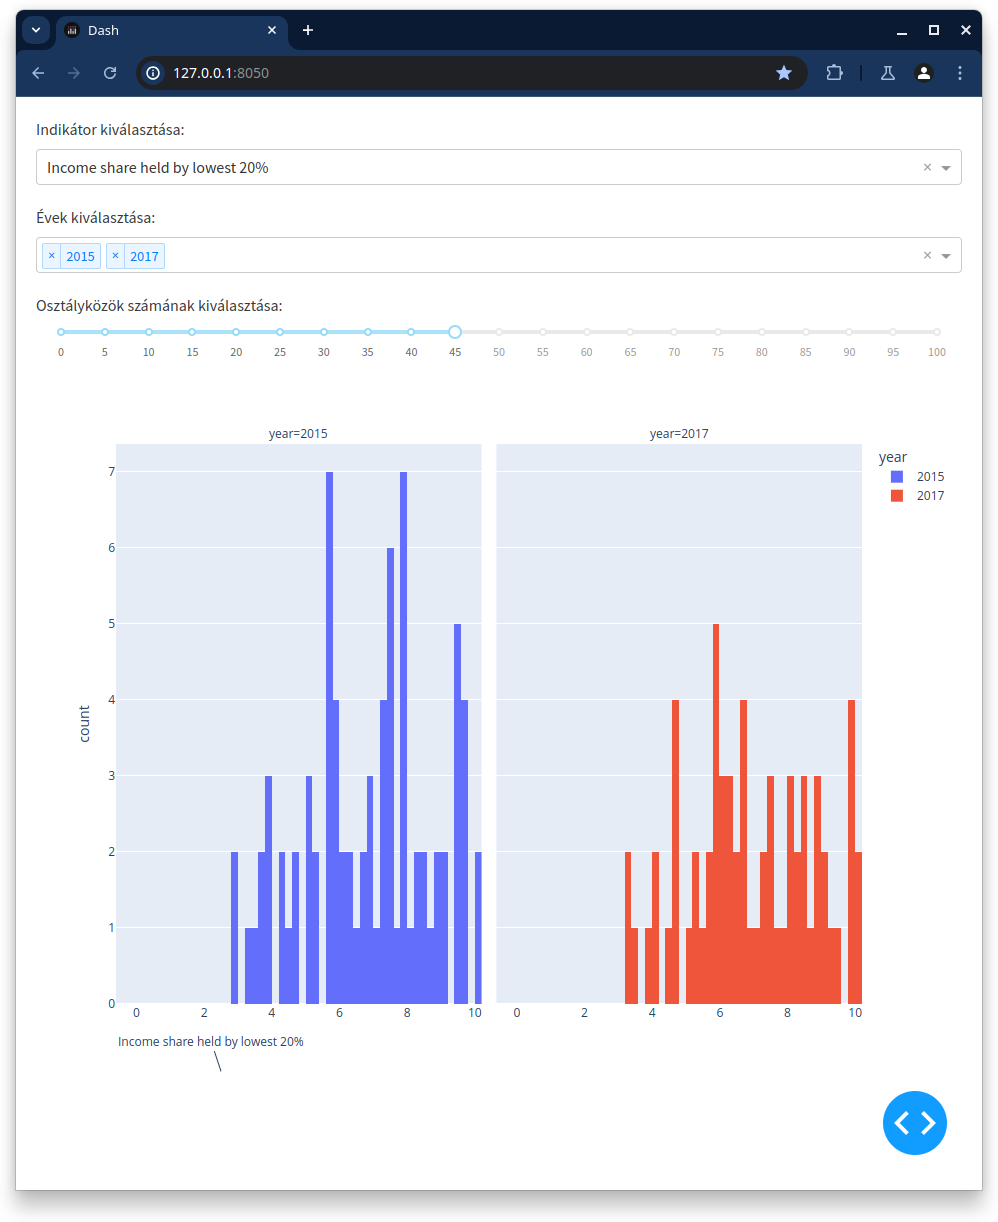
\includegraphics[width=7cm, height=7cm, keepaspectratio]{images/freq_9.png}
			\end{center}
		\end{column}
	\end{columns}
\end{frame}

\end{document}










